\documentclass{article}% [Determines font size] { }Determines type of document (article/beamer/book/etc.)

\usepackage{graphicx}% Required package to compile figures.
\usepackage{blindtext}

\begin{document}% Required to produce a compiled LaTeX document. 

\blindtext

\begin{figure}[!b]% "b" is used to place at the bottom of the document, but since there is too much text without a break in the environment, LaTeX can't fit the figure where it's being specified. But adding the "!" forces the break in the environment and pushes the remaining text to the next page.  
        \caption{Complete figure format}%
        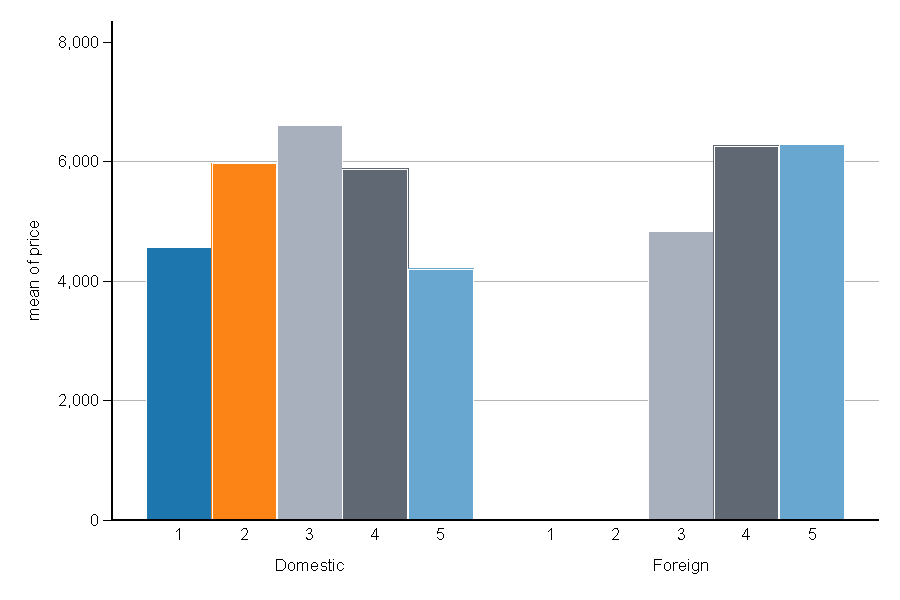
\includegraphics[width=1\textwidth]{figure1.pdf}% 
        \label{fig:placement_!b}%
\end{figure}

\blindtext[4]

\newpage

\blindtext

\begin{figure}[b]% This demonstrates what happens if in the previous scenario there was no exclamation point used.
        \caption{Complete figure format}% 
        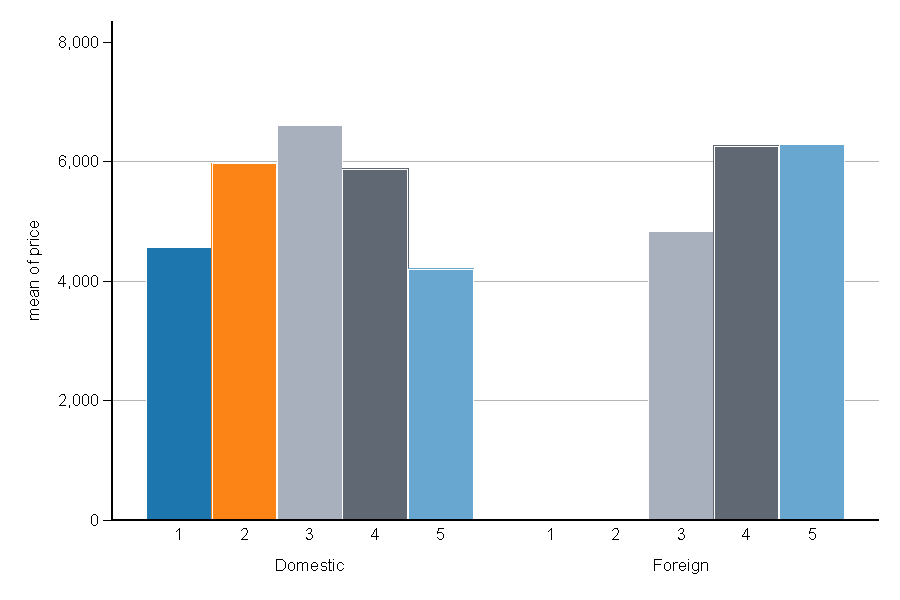
\includegraphics[width=1\textwidth]{figure1.pdf}% 
        \label{fig:placement_b}%
\end{figure}

\blindtext[4]

\end{document}